\section{Merge}

\subsection{C}
El código de C es bastante simple. Lo que hace al inicio es convertir ambos punteros a punteros a matrices de matrices, que tienen elementos de $w$ bytes de tamaño, que a su vez tienen elementos de 4 bytes de tamaño.

Luego se realizan 3 ciclos, el primero sobre las filas, el segundo sobre las columnas, y el tercero sobre los canales (exceptuando el canal de transparencia, notar que ii se inicializa en 1).

Finalmente se realiza la cuenta que se debe hacer para hacer el merge, convirtiendo todo adecuadamente (se convierte el valor del canal, que es un entero de 1 byte a float, se lo multiplica por value o 1-value según corresponda, se lo suma con el otro valor y se lo vuelve a convertir a entero de 8 bytes).

\subsection{ASM1}

En la primera versión del código de ASM, iniciamos guardando los parámetros que nos pasan en algunos registros auxiliares para no perderlos mas adelante.
Luego calculamos h*w dado que es la cantidad de iteraciones que vamos a realizar.

En el ciclo lo que hacemos es tener dos vectores de floats

\xmm{3}
\regfloats{$value$}{$value$}{$value$}{$1.0$}

\xmm{4}
\regfloats{$1-value$}{$1-value$}{$1-value$}{$0.0$}

Y levantamos de a un píxel, cuyos canales convertimos a float y multiplicamos por los registros exhibidos anteriormente. Luego convertimos a enteros de 8 bits nuevamente, empaquetando.

Notar que no se produce overflow. Tomemos por ejemplo el canal R, y supongamos que el valor del canal R para ambas imágenes es $255$.
Entonces $255value + 255(1-value)$ da $255$, que entra en 8 bits (si por errores de redondeo diera más, no importa, ya que el empaquetado lo hacemos saturado, entonces se queda en 255).

Finalmente escribimos en el lugar de la memoria correspondiente el valor obtenido y listo, repetimos este proceso hasta terminar.

Aunque en líneas generales esta rutina es igual a la de C, esperamos que tenga mejor rendimiento por dos razones.
Primero, en esta rutina tenemos que hacer menos saltos, dado que solo tenemos un ciclo, mientras que la versión de C tiene 2 ciclos.
Segundo, porque si el compilador no optimiza a la perfección las operaciones, es muy probable que realice las operaciones de los canales en serie, en vez de como lo hacemos nosotros, en paralelo.
Es decir, en el código de C los canales se van a procesar uno detrás del otro, mientras que en nuestro código se van a procesar todos juntos.


\subsection{ASM2}

Al igual que en la rutina anterior, luego de armar el stack frame guardamos los parámetros en algunos registros auxiliares para no perderlos. El resto del proceso es el mismo que antes, hasta que llegamos al precalculo de los vectores de $value$. Como aquí hay que hacer operaciones con enteros, en vez de punto flotante como antes, vamos a calcular las cosas de manera diferente.

En vez de guardarnos $value$, vamos a guardarnos $int16(256*value)$. ¿Por qué? Porque de esta manera vamos a poder cargar de a dos píxeles y hacer las operaciones mucho mas rápido que antes. Además así guardamos un valor que antes estaba entre 0 y 1 en un valor que esta entre 0 y 256, es decir, un valor que podemos representar con una buena aproximación entera.

De esta manera nos armamos el vector igual que antes, solo que multiplicado por 256. Luego lo pasamos a entero y luego lo empaquetamos consigo mismo en la parte alta.

De esta manera obtenemos en \xmm{3} los siguientes valores

\xmm{3}
\regintOcho{256$v$}{256$v$}{256$v$}{256}{256$v$}{256$v$}{256$v$}{256}

Donde $v$ es $value$.


Ahora, nos gustaría tener en el otro registros los números tal que, sumados con los de \xmm{3}, dan 256. Para eso, nos aprovechamos de la representación complemento a 2, dado que lo que queremos en realidad son los inversos aditivos (en 8 bits) de estos números en el registro \xmm{4}. Entonces usamos que el inverso aditivo de un número es el negado bit a bit más 1.

Cargamos en \xmm{4} 8 enteros de 16 bits con valor 257, ya que es 256+1.
Luego, al hacer la diferencia

\begin{lstlisting}
psubw xmm4, xmm3
\end{lstlisting}

obtenemos en \xmm{4} exactamente lo que queremos, es decir que si sumamos int16 a int16 en \xmm{3} y \xmm{4} da 256. Luego comenzamos el ciclo principal, que es muy similar al anterior.

Viendo esta implementación creemos que su desempeño va a ser aún mejor que el de la primera implementación en Assembler, dado que hacemos operaciones con números enteros que son mucho más rápidas que las operaciones con punto flotante. Sin embargo, hacer operaciones con números enteros implica un trade-off de velocidad por precisión, aunque el código es mucho mas rápido también es (muy poco) más inexacto. Analizaremos este error a continuación.

\subsubsection{Error}

En la segunda versión de merge se comete, obviamente, más error que en la primera, dado que estamos trabajando con enteros, debemos perder precisión cuando convertimos $256v$ a entero.

Por esta razón, aproximadamente el 30\% de las veces, el resultado difiere en más de 2 con el output de C de la cátedra. Esto se debe a que los métodos de cómputo son fundamentalmente distintos, uno con mucha mas precisión que la otra.

Pese a esto, el 100\% de los tests pasan con un error de 3, es decir, pese a que existe error, es despreciable. El error (por ejemplo, para el canal R) se puede expresar de la siguiente manera

$$\bigg|\lfloor R_1v\rfloor + \lfloor R_2(1-v) \rfloor
  -\bigg\lfloor \frac{R_1\lfloor 256v \rfloor}{256} \bigg\rfloor 
 -\bigg\lfloor \frac{R_2(256- \lfloor 256v) \rfloor)}{256} \bigg\rfloor\bigg| $$


$$\leq
\bigg|
\lfloor R_1v\rfloor - \bigg\lfloor \frac{R_1\lfloor 256v \rfloor}{256} \bigg\rfloor
\bigg|
+
\bigg|
\lfloor R_2(1-v) \rfloor -\bigg\lfloor \frac{R_2(256- \lfloor 256v) \rfloor)}{256} \bigg\rfloor
\bigg| $$

Se puede verificar fácilmente con Wolfram-Alpha o algún software similar que es es menor que 3.


\pagebreak

\subsection{Experimentación}

Antes de comenzar a testear, supusimos que la performance de nuestros programas en Assembler iban a ser muy superiores a las de C. Creemos esto dado que vamos a aprovecharnos mejor de las utilidades de SSE que lo que puede hacer un compilador. 

Esperamos también que la performance mejore aún más en la segunda implementación, dado que todas las operaciones las realizamos con enteros en vez de con punto flotante.


\begin{figure}[!hbt] 
  \centering
  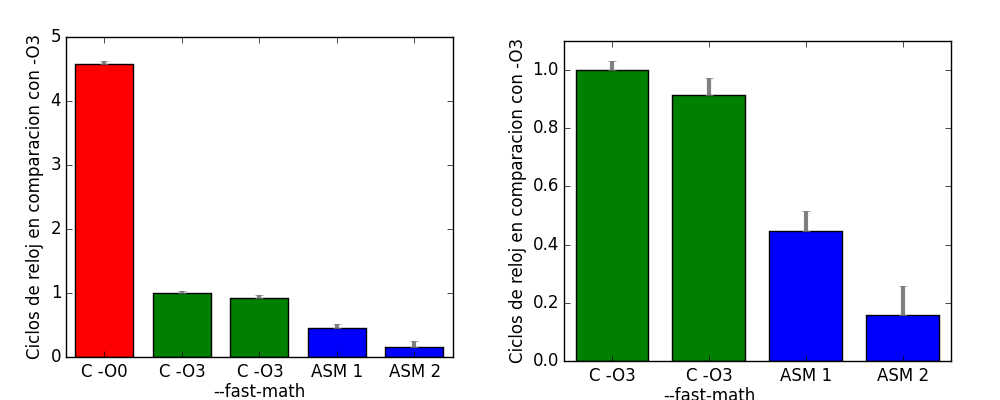
\includegraphics[scale=0.7]{merge-all.png}
  \caption{Comparación de la cantidad de ciclos de reloj utilizada por diferentes variantes de merge. Para tener una medida absoluta: la cantidad de ciclos de reloj promedio de C -O3 es 4,293,199. Tamaño de la muestra: 200 imagenes de $16 \times 10^4$ píxeles. Se indica el mínimo con la barra y el promedio con una linea gris.}
\end{figure}


Viendo los resultados, confirmamos nuestras hipótesis. De hecho, la performance de nuestros programas son mejores que las esperadas.

Como puede verse en los gráficos de escalabilidad, la performance de todos los algoritmos depende linealmente de la cantidad de píxeles de la imagen, sin embargo lo que cambia entre las diferentes implementaciones es la pendiente de esta función lineal.

La performance no depende de la imagen, dado que la operación que se realiza siempre es la misma, sin depender de los píxeles en cuestión.
Sin embargo, hay una cuestión con el error. Si el $\alpha$ que nos pasan por parámetro tiene muchos decimales detrás de la coma, es muy probable, y de hecho pasa, que nuestra segunda implementación en Assembler pierde precisión frente a la implementación de C. Esto fue explicado anteriormente, sin embargo creímos pertinente nombrarlo.

La única mejora que se nos ocurre para el código propuesto de Assembler es, si supiéramos que el inicio de la matriz está alineado a 16 bytes, entonces podríamos levantar de a 4 píxeles y analizarlos todos juntos (haciendo una especie de ciclo unrolling, es decir, teniendo 4 ciclos normales dentro de 1).
Esto es posible que mejore la performance, sin embargo es necesario como precondición que la matriz esté alineada a 16 bytes, ya que si no lo está y usamos una instrucción para leer alineado, los resultados serán desastrosos.

La comparación entre el programa de C y el de Assembler no es lo suficientemente justa. Esto se debe a que la versión de C por cada píxel, tiene 3 accesos a memoria, mientras que nuestra implementación tiene un acceso a memoria por píxel. Esto genera obviamente un speedup enorme, sobre todo en computadoras con memoria de velocidad limitada.
Aunque es posible que la gran mayoría de los accesos sean a cache, la performance ganada es significativa.

El acceso a memoria en nuestros códigos de Assembler es lo mínimo indispensable. La única mejora que se podría hacer con respecto al acceso a memoria es lo que fue nombrado anteriormente es la idea de hacer un unroll del ciclo y leer de a 4 píxeles, pero creemos que la performance no mejorará significativamente.

La diferencia entre operar con punto flotante y con enteros es significativa. Aunque ambas implementaciones en Assembler son mucho mas rápidas que la implementación de C, la que opera con enteros es nuevamente (bastante) más rápida que la que opera con punto flotante. Esto se debe a que en general las operaciones con enteros son mucho mas rápidas que las de punto flotante.



